\section{Lippukunnanjohtajan tervehdys}

\begin{multicols}{2}
\noindent Haarapääskyt, räystäspääskyt ja tervapääskyt ovat jo aikaa sitten
saapuneet, merihanhilla on jo poikasia ja kuuluipa pellon laidalta
tuttu harmaasiepon ''tsri tsri tsri''. Kevät on jo täällä ja kesä on
aivan kulman takana. Valkovuokko, rentukka ja kirsikka ovat täydessä
kukassa ja ensimmäiset satakielet virittävät lauluaan aamuhämärässä.
Aivan, kesällä järjestetään lippukunnan \textit{Satakieli}"-kesäleiri!
Leirin lisäksi kesän toimintaan lukeutuvat \textit{Variksen vavahdus}
"=vaellus ja \textit{Piisaminhäntä}"-melonta. Olethan sinäkin mukana
kesän partiotapahtumissa?

Alkuvuoteen on jälleen mahtunut monenlaista partiotekemistä kuten
laskiaisriehaa, minihaikkia, partioparaatia ja lippukuntaretkeä. Olen
haltioissani siitä, kuinka paljon erilaista toimintaa pieni
lippukuntamme on pystynyt järjestämään; kevään toimintamme on
kartuttanut käyntikertoja yli seitsemänsataa! Tämä ei ole mikään
itsestäänselvyys, vaan mielekäs toiminta vaatii aina vapaaehtoisia,
tekijöitä ja johtajia -- unohtamatta itse osallistujia, joita ilman
tekeminen menettää merkityksensä.  

Osin partiotoiminnan mahdollistaa se, että lippukuntamme on
rekisteröity yhdistys. Sillä on vuosikokouksen valitsema hallitus, joka
vastaa toimintasuunnitelman toteutumisesta, päättää kalusto- ja muista
hankinnoista, ylläpitää jäsenrekisteriä, anoo avustuksia, edustaa
lippukuntaa piirin aluetapaamisissa\ldots\ Lippukunnan hallinto on
yleistäen kuin valtion, kunnan tai jonkin yrityksen hallinto
pienoiskoossa, joten partiotoiminnan tähän välillä tylsältäkin
vaikuttavaan osaan tutustuminen tarjoaa johtajalle paljon hyödyllisiä
tietoja ja taitoja, joista on aikuisena hyötyä muuallakin. Haluaisitko
sinä tutustua lippukunnan hallituksen tehtäviin? Kysy lisää
allekirjoittaneelta!

Tässä Tassussa pääset palaamaan viime vuoden pikkujouluretkeen,
riihitystunnelmiin vuonna 2018 ja tänä keväänä sekä tarpojien
minihaikille. Seikkailijoiden sivuilla (s. \pageref{sec:seikkailijat})
on paljon hauskaa luettavaa ja tekemistä. Julkistetaanpa lehdessä myös
viime numeron kuvakilpailun voittaja. Ja jos et ole vielä aloittanut,
nyt on oikea hetki alkaa pohtia, kuinka oikea ja nurja silmukka oikein
tehtiinkään, ottaa neulepuikot esiin ja osallistua Tassun
neulesuunnittelukilpailuun -- lue lisää sivulta
\pageref{sec:neulekilpailu}!

{\smallskip\noindent\centering ***\par\smallskip}

Kevättä varjosti Kurkisuon Rusakoiden perustajajäsenen ja ensimmäisen
lippukunnanjohtajan, \mbox{Eddien} poisnukkuminen. ''Yritä jättää tämä
maailma vähän parempana kuin sen löysit,'' kehotti lordi Baden"-Powell,
partioliikkeen perustaja viimeisessä viestissään maailman
partiolaisille. Sama ilmaisu löytyy Suomen Partiolaisten
partioneuvoston hyväksymistä partion yhteiskunnallisen toiminnan
linjauksista. Nykyisenä lippukunnanjohtajana olen vahvasti sitä mieltä,
että Eddie otti kehotuksesta vaarin.

Partioterveisin ja Eddien muistoa kunnioittaen

\smallskip

\noindent\hfill Janne

\vspace*{12cm}

\columnbreak

\null\vfill

\noindent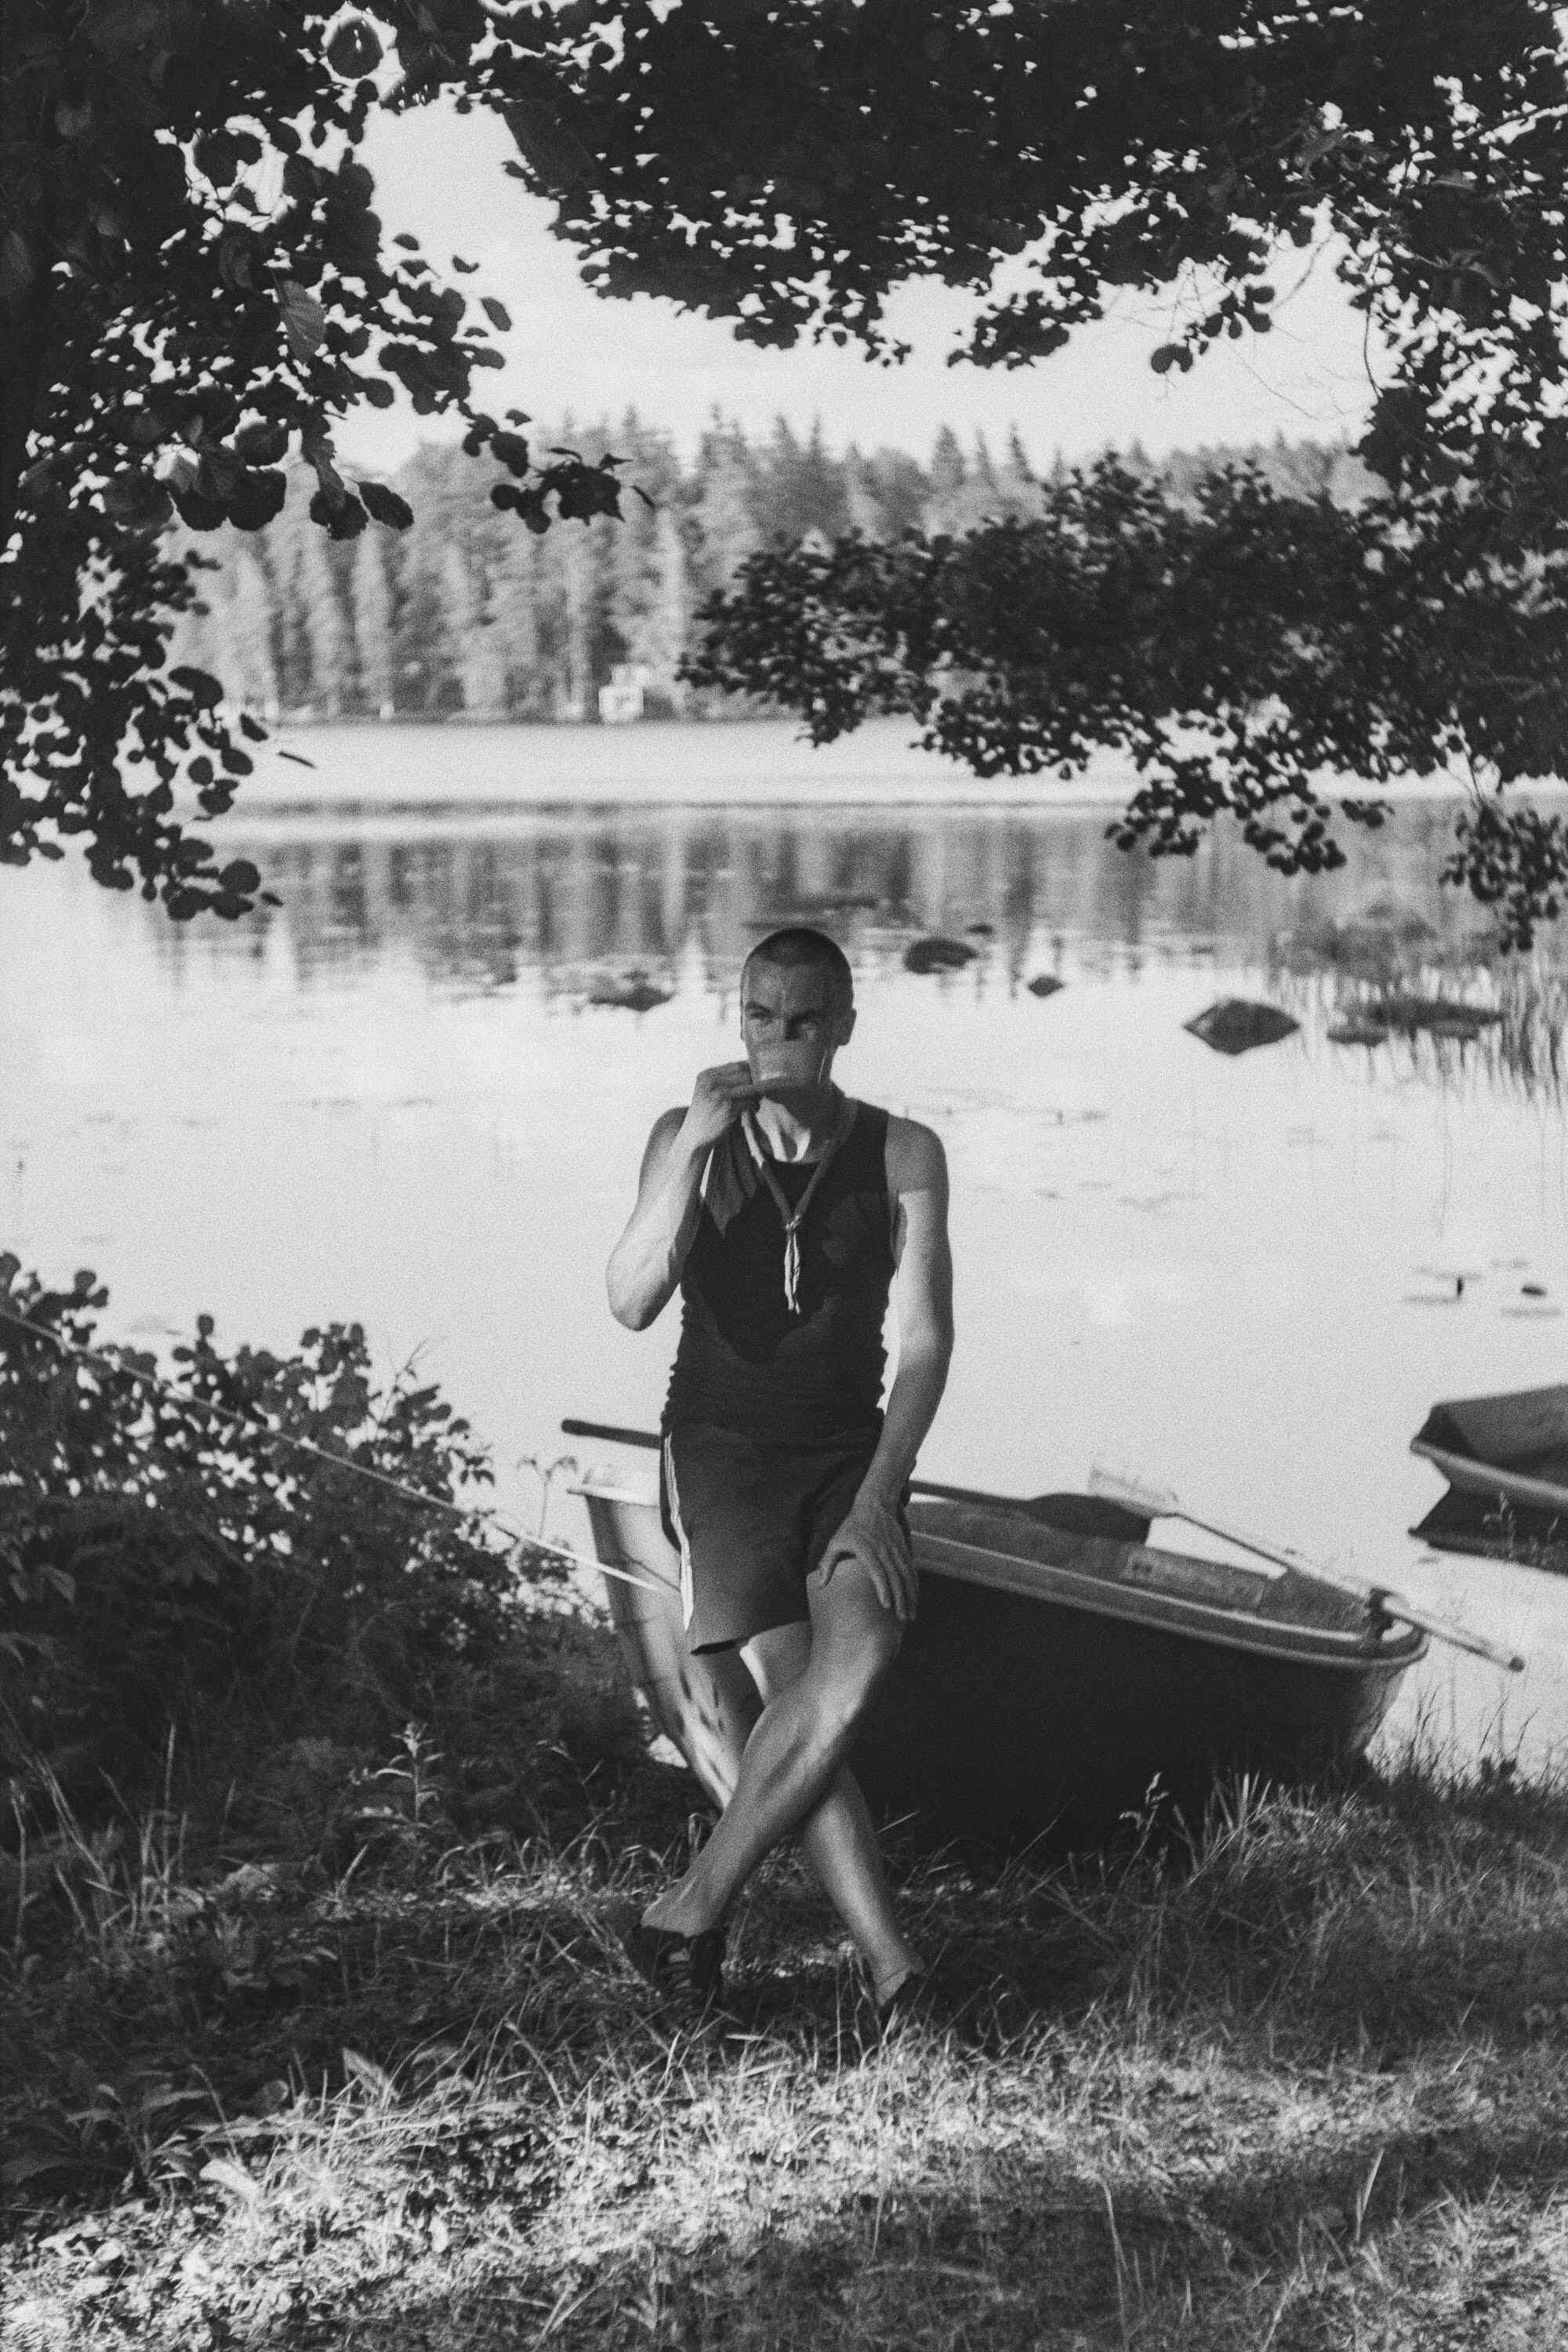
\includegraphics[width=\linewidth]{assets/lpkjohtajantervehdys} \\
{\small Lippukunnanjohtaja nauttimassa iltateestä \textit{Uikun uinti}
"=vaelluksen helteisen, kolmannen päivän päätteeksi Ruokojärven rannalla.\par}

\bigskip

\noindent\null\hfill Kuva: Tanguy
\end{multicols}
